% WACV 2024 Paper Template
% based on the CVPR 2023 template (https://media.icml.cc/Conferences/CVPR2023/cvpr2023-author_kit-v1_1-1.zip) with 2-track changes from the WACV 2023 template (https://github.com/wacv-pcs/WACV-2023-Author-Kit)
% based on the CVPR template provided by Ming-Ming Cheng (https://github.com/MCG-NKU/CVPR_Template)
% modified and extended by Stefan Roth (stefan.roth@NOSPAMtu-darmstadt.de)

\documentclass[10pt,twocolumn,letterpaper]{article}

%%%%%%%%% PAPER TYPE  - PLEASE UPDATE FOR FINAL VERSION
% \usepackage[review,algorithms]{../wacv}      % To produce the REVIEW version for the algorithms track
%\usepackage[review,applications]{wacv}      % To produce the REVIEW version for the applications track
\usepackage{wacv}              % To produce the CAMERA-READY version
%\usepackage[pagenumbers]{wacv} % To force page numbers, e.g. for an arXiv version

% Include other packages here, before hyperref.
\usepackage{graphicx}
\usepackage{amsmath}
\usepackage{amssymb}
\usepackage{booktabs}

\usepackage{times}
\usepackage{epsfig}
\usepackage{epsf}
\usepackage{subcaption}
\usepackage{placeins}
\usepackage{paralist}
\usepackage{textcomp}
\usepackage{xr}

% Include other packages here, before hyperref.
\externaldocument[Paper-]{petit_wacv}

% It is strongly recommended to use hyperref, especially for the review version.
% hyperref with option pagebackref eases the reviewers' job.
% Please disable hyperref *only* if you encounter grave issues, e.g. with the
% file validation for the camera-ready version.
%
% If you comment hyperref and then uncomment it, you should delete
% ReviewTempalte.aux before re-running LaTeX.
% (Or just hit 'q' on the first LaTeX run, let it finish, and you
%  should be clear).
\usepackage[pagebackref,breaklinks,colorlinks]{hyperref}


% Support for easy cross-referencing
\usepackage[capitalize]{cleveref}
\crefname{section}{Sec.}{Secs.}
\Crefname{section}{Section}{Sections}
\Crefname{table}{Table}{Tables}
\crefname{table}{Tab.}{Tabs.}


%%%%%%%%% PAPER ID  - PLEASE UPDATE
\def\wacvPaperID{1891} % *** Enter the WACV Paper ID here
\def\confName{WACV}
\def\confYear{2024}


\begin{document}
\setcounter{section}{5} % set the section counter to the last section number in the main paper
\setcounter{equation}{15} 
\setcounter{figure}{4}

%%%%%%%%% TITLE
\title{PETIT-GAN Supplementary Material}
\maketitle


\section{Physical estimator coefficient calibration}
\label{sec:calibration}
This section provides a more detailed description of the physical estimator calibration procedure described in sub-subsection \ref{Paper-subsubsec:calibration} of the paper.

Equation \ref{Paper-IntensityVsTemperatures} provides a parametric model that allows us to transform thermal image intensities to object temperatures and vice versa.
To calibrate those parameters, we designed a calibration setup with the following components:
\begin{itemize}
  \item an uncooled microbolometric camera; for our experiments, we used FLIR Tau2.
  \item an environmental chamber to control the camera's ambient temperature (which implicitly controls $T_\mathit{int}$), with an aperture drilled into one of its edges to allow for image acquisition from its interior.
  \item a blackbody target, essentially a flat-surface object whose temperature can be controlled with very fine precision, to set the temperature of the scene (\ie, $T_\mathit{obj}$);
  we used a scientific grade (CI SR-800N) extended-area black body.
\end{itemize}
To collect measurements, the camera was mounted inside the environmental chamber, facing outside through the drilled aperture, and the blackbody target was placed in front of the camera outside the chamber, such that it covered the camera's entire field of view, as demonstrated in Figure \ref{calib_setup}.

\begin{figure}
  \centering
  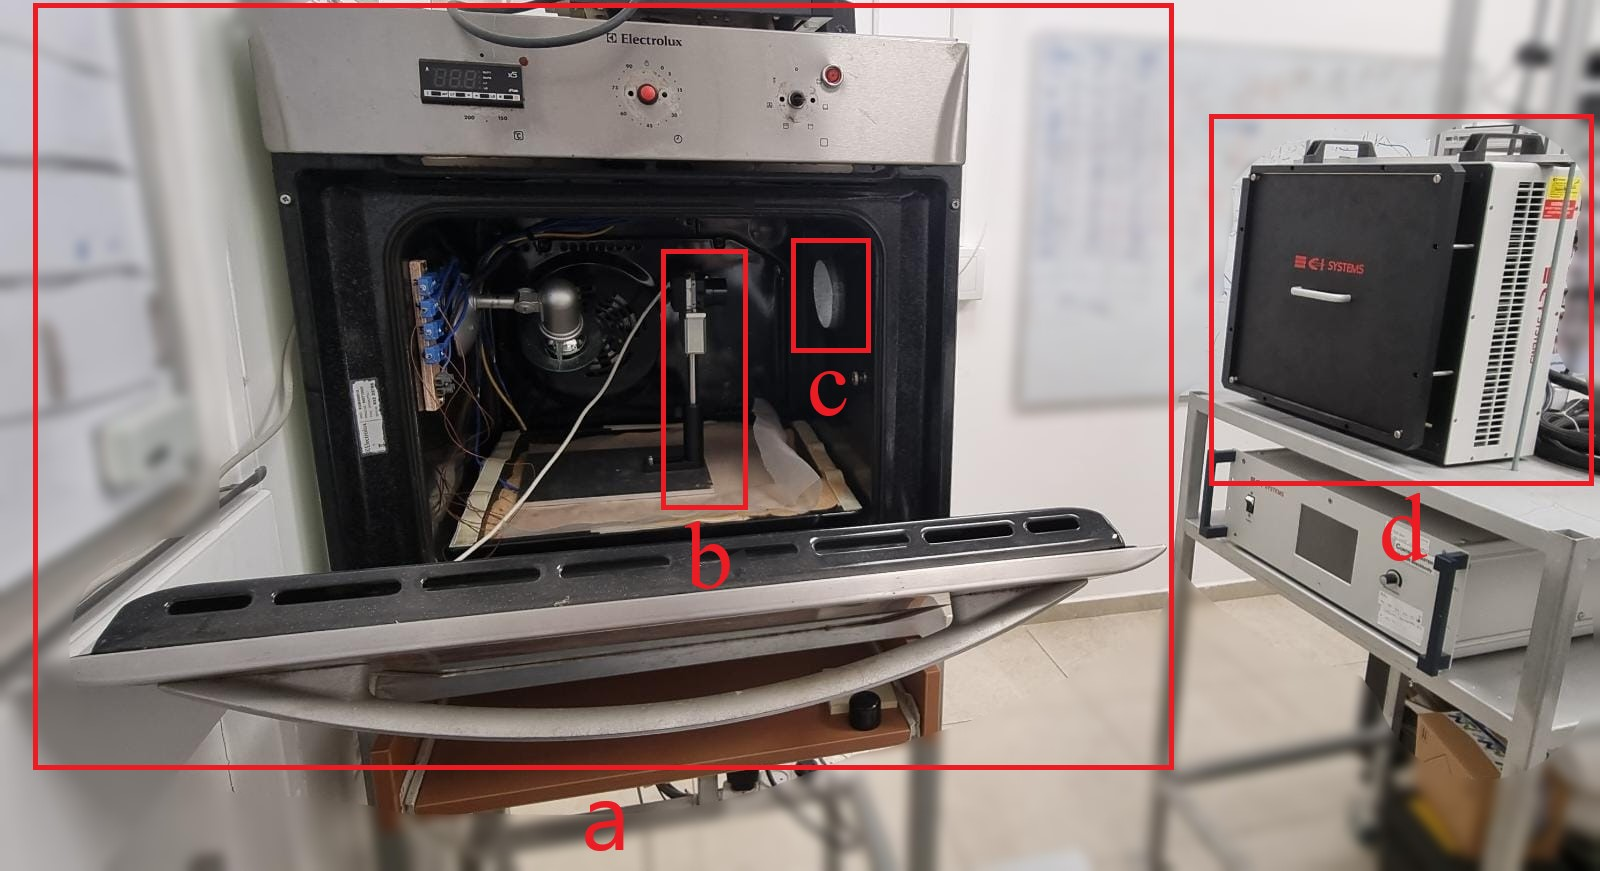
\includegraphics[width=\linewidth]{../figs/methods/calib_setup.jpg}
  \caption{The physical model-calibration setup. The black body target (d) is observed by the thermal camera (b) through a drilled aperture (c) at the edge of the environmental chamber (a). This setup enables controlling $T_\mathit{obj}$ and $T_\mathit{int}$ independently.}
  \label{calib_setup}
\end{figure}

During the calibration, the environmental chamber is set for heating (thus slowly and continuously increasing $T_\mathit{int}$). 
While the chamber's interior ambient temperature keeps increasing, the blackbody target is repeatedly set to an arbitrary temperature, and an image is acquired for every such temperature.
This random target-temperature profile provides the best coverage of the three-dimensional $T_\mathit{int}$-$T_\mathit{obj}$-intensity space compared to other alternatives.


To efficiently estimate the coefficients, we organized the measured intensities and the coefficients in vectors $I$ and $C$ correspondingly, such that:
\begin{equation} \label{eq:matMult}
  M \cdot C = I
\end{equation}
where each row of the over determined matrix $M$ is the feature vector ($F$) of a single measurement, and $I$
holds the corresponding measured radiometric intensities.
Following the factorization from equation \ref{Paper-eq:full_expr}, the $n$th measured radiometric intensity equals the inner product between the $n$th measured feature vector and the vector of coefficients $C$:
\begin{equation}
  I[n] = <M[n, :], C> = <F[n], C>
\end{equation}
The matrix product factorization in equation \ref{eq:matMult} enables applying a linear regression to solve for the coefficients.
As the measurement noise appeared to be approximately white and Gaussian, the least-squares estimator (which is the maximum-likelihood estimator in the additive-white-Gaussian noise regime) was used to extract the coefficients:
\begin{equation} \label{eq:PseudoInverse}
  C = M^{\dagger} I
\end{equation}
where $M^{\dagger} = (M^TM)^{-1}M^T$ is the Moore-Penrose pseudoinverse of $M$.

In the calibration process described above, the intensity vector $I$ corresponds to measurements of a single pixel.
Because each element in the microbolometer might have a different sensitivity, the coefficient extraction was performed independently for every pixel in the image.


\section{Dataset}
As mentioned in subsection \ref{Paper-sec:dataset} of the paper, one of our contributions is the introduction of a novel dataset of unpaired images belonging to different bands of the thermal (LWIR) spectrum.
In the discussed subsection, we provided a brief description of the data collection procedure.
This section provides more details about the dataset, including the data collection, the data format, and the preprocessing applied to the data.
The dataset can be accessed through the \href{https://bermanz.github.io/PETIT/}{project's website}.

\subsection{Data collection}
In the paper's introduction, we presented the motivation of our research - synthesizing a multispectral dataset to allow the development of algorithms and systems for nanosatellites.
Thus, our goal was to mimic the interstellar acquisition setup to the best pf our ability.
To that end, a light airplane (appears in Figure \ref{fig:light_airplane}) was used to perform flights at a height of approximately two kilometers above ground.
Images acquired in such a setup could be later reasonably extrapolated, \eg, by a proper downsampling, to mimic the scene as if it was captured by an actual nanosatellite.
\begin{figure}[h]
    \centering
    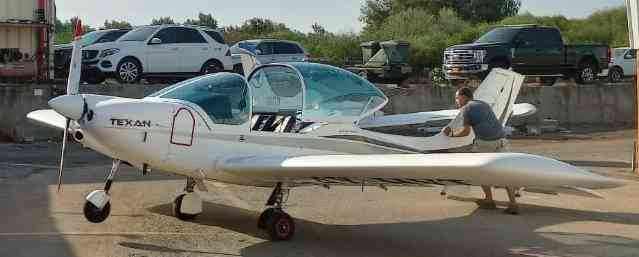
\includegraphics[width=0.8\linewidth]{../figs/data/light_airplane.jpeg}
    \caption{The light airplane used for acquiring the thermal images.}
    \label{fig:light_airplane}
\end{figure}

A dedicated aerial pod was designed and manufactured to mount the camera on the airplane's underbelly, as visualized in Figure \ref{fig:camera_jig}.
\begin{figure}[h]
    \centering
    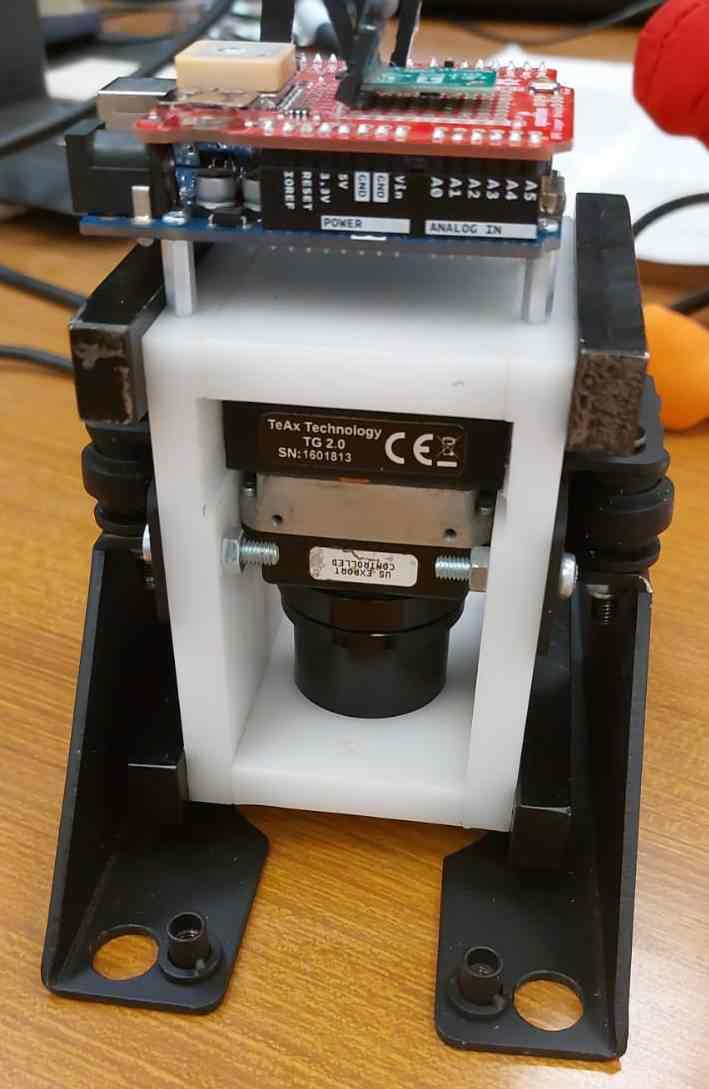
\includegraphics[width=0.1\textwidth]{../figs/data/camera_jig_actual.jpeg}
    \caption{The aerial pod used for mounting the thermal camera on the light airplane's underbelly.}
    \label{fig:camera_jig}
\end{figure}

The pilot performed several flights, with some IR bandpass filter applied to the camera lens (monochromatic), or without this filter (panchromatic).
While attempting to follow the same predefined trajectory, ensuring that the actual airplane's positional and angular states are the same for different flights is physically infeasible.
Jittering and air bumps provide additional randomness to the system's state, resulting in unpredictable and unreproducible acquisition conditions.
Due to those limitations, the images collected for the different thermal modalities are inherently unpaired, hence our entire dataset is unpaired.

\subsection{Data format}
Each frame in the dataset is saved as an independent numpy \emph{.npz} file with the following fields:
\begin{itemize}
    \item \emph{image}: a two-dimensional $256 \times 336$ Numpy array containing the radiometric intensities acquired by the Flir TAU2 camera (with 14-bit precision).
    \item \emph{time}: the date and time of the acquired image in GMT.
    \item \emph{lat}: the latitude of the plane at the time of acquisition. 
    \item \emph{long}: the longitude of the plane at the time of acquisition. 
    \item \emph{alt}: the altitude of the plane above sea-level at the time of acquisition (in meters).
    \item \emph{fpa}: the intrinsic temperature of the camera as measured by the focal-plane array thermal sensor (in Celsius).
\end{itemize}

\subsection{Preprocessing}
Due to technical considerations, a significant portion of the acquired images were purely of sea with no additional features.
Pure-sea images are roughly thermally homogeneous, \ie, of a constant intensity level, up-to measurement noise and spatial aberrations, making them extremely similar to each other and of lesser value to our training.
Naively using all those images for training a would result in a highly imbalanced dataset, which will bias our model to produce high quality outputs for sea images, in the expense of other samples.
An impression of the described attributes of sea images can be obtained from Figure \ref{fig:sea_image}.
\begin{figure}[ht]
    \begin{subfigure}[b]{0.23\textwidth}
        \centering
        
\includegraphics[width=\textwidth]{../figs/data/sea.png}
        \subcaption*{Sea}
        \label{fig:sea}
    \end{subfigure}
    \hfill
    \begin{subfigure}[b]{0.23\textwidth}
        \centering
        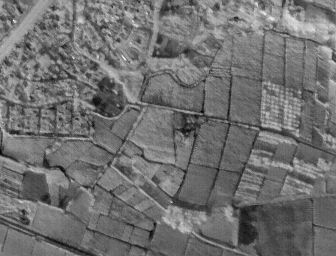
\includegraphics[width=\textwidth]{../figs/data/land.png}
        \subcaption*{Land}
        \label{fig:land}
    \end{subfigure}
    \hfill
    \caption{A thermal image of pure sea \vs an image of land for reference.}
    \label{fig:sea_image}
\end{figure}

For those reasons, it was decided to design a classifier for filtering out all sea images from the dataset.
As explained and visualized, sea images are mostly made out of a DC component (constant) and measurement noise.
This means that the gradients of two images of sea, even at different water temperatures, should have a very similar high-frequency spectral content.
Analyzing the gradients of sea and land images confirms this hypothesis, as demonstrated in Figure \ref{fig:grad_img_comp}.
\begin{figure}[ht]
    \begin{subfigure}[b]{0.15\textwidth}
        \centering
        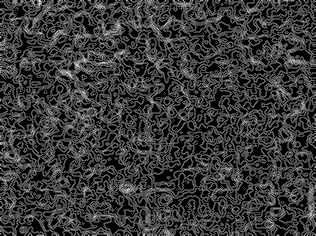
\includegraphics[width=\textwidth]{../figs/data/sea_grad-ref.png}
        \subcaption*{Sea Reference}
        \label{fig:sea_grad-ref}
    \end{subfigure}
    \hfill    
    \begin{subfigure}[b]{0.15\textwidth}
        \centering
        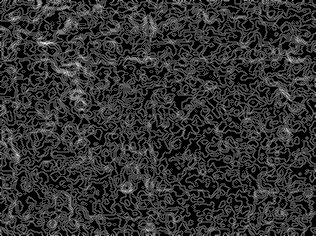
\includegraphics[width=\textwidth]{../figs/data/sea_grad.png}
        \subcaption*{Sea}
        \label{fig:sea_grad}
    \end{subfigure}
    \hfill
    \begin{subfigure}[b]{0.15\textwidth}
        \centering
        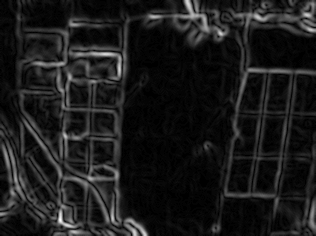
\includegraphics[width=\textwidth]{../figs/data/land_grad.png}
        \subcaption*{Land}
        \label{fig:land_grad}
    \end{subfigure}
    \caption{The gradient maps of exemplary land and sea images. An additional gradient map of a sea image is provided for reference.}
    \label{fig:grad_img_comp}
\end{figure}
This finding encouraged us to base our classifier upon the gradients of the images.
A more thorough quantitative analysis of the gradients revealed a significant difference between the norms of the gradients of sea and ground images.
This difference is also visible in Figure \ref{fig:gradients_norm} where the norms of ten randomly-selected sea and land images are compared.
\begin{figure}[ht]
    \centering
    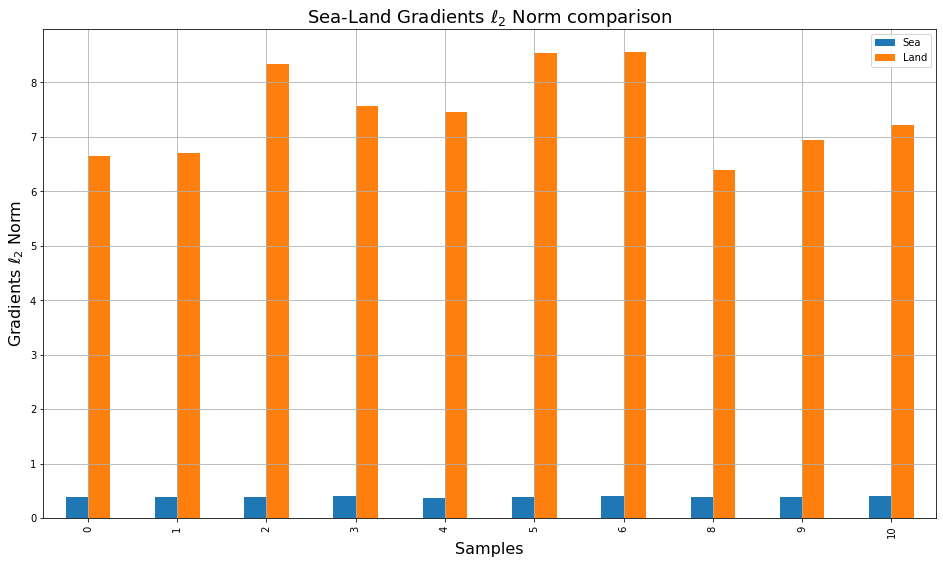
\includegraphics[width=\linewidth]{../figs/data/grad_norm_comp.png}
    \caption{A histogram of the $\ell_2$ norm of the gradients of random sea and land images taken from the dataset.}
    \label{fig:gradients_norm}
\end{figure}

Following these findings, the following pipeline was designed:
\begin{enumerate}
    \item Prefiltering of the acquired image $I$ with a two-dimensional gaussian low-pass filter to attenuate the noise and very high frequencies, which typically don't belong to the spectral content of natural images. 
    We denote our filtered image by $\tilde{I}$.
    \item Classify $I$ as a land image if $||\nabla \tilde{I}||_2$ (the $\ell_2$ norm of the gradient of $\tilde{I}$) is greater than some threshold $\tau$, and otherwise as a sea image. 
\end{enumerate}
The threshold's value $\tau$ was set to the average between the minimum $\ell_2$ norm of the gradients over a random set of 1000 land images and the maximum $\ell_2$ norm of the gradient over a random set of 1000 sea images.
Formally:
\begin{equation}
    \tau = \frac{1}{2} \left( \underset{I_\mathit{l} \in D_\mathit{land}}{min} ||\nabla I_\mathit{l}||_2 
    + \underset{I_\mathit{s} \in D_\mathit{sea}}{max} ||\nabla I_\mathit{s}||_2 \right)
\end{equation}
The entire preprocessing pipeline, as well as the calibrated threshold, were designed and applied to both monochromatic and panchromatic images independently.

\section{Additional qualitative results} \label{sec:additional_res}
Following our guarantee from sub-subsection \ref{Paper-subsubsec:qual_res}, we provide additional qualitative examples of our model's output. 
These additional examples provide additional evidence to the claim made in the paper regarding our model's superior quality compared to the baseline models.
All additional examples appear in Figure \ref{fig:qual_res_sup} in the page below.
\cleardoublepage

\onecolumn
\begin{figure*}[!ht]
  % 1st Row
  \centering
  \begin{subfigure}[b]{0.19\textwidth}
      \centering
      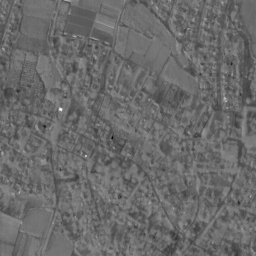
\includegraphics[width=\textwidth]{../figs/outputs/pan/2.png}
  \end{subfigure}
  \hfill
  \begin{subfigure}[b]{0.19\textwidth}
      \centering
      
\includegraphics[width=\textwidth]{../figs/outputs/cycleGan/2.png}
  \end{subfigure}
  \hfill
  \begin{subfigure}[b]{0.19\textwidth}
      \centering
      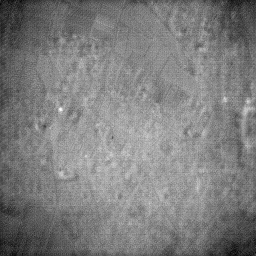
\includegraphics[width=\textwidth]{../figs/outputs/cut/2.png}
  \end{subfigure}
  \hfill
  \begin{subfigure}[b]{0.19\textwidth}
      \centering
      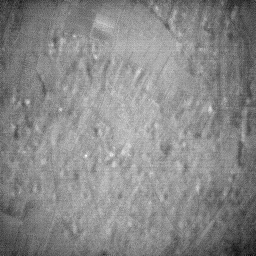
\includegraphics[width=\textwidth]{../figs/outputs/petit/2.png}
  \end{subfigure}
  \hfill
  \begin{subfigure}[b]{0.19\textwidth}
      \centering
      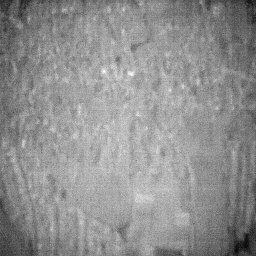
\includegraphics[width=\textwidth]{../figs/outputs/mono/230.png}
  \end{subfigure}      
  
  % 2nd Row
  \centering
  \begin{subfigure}[b]{0.19\textwidth}
      \centering
      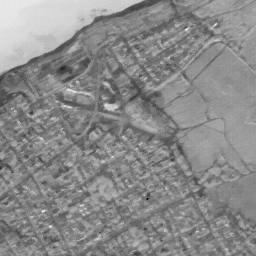
\includegraphics[width=\textwidth]{../figs/outputs/pan/3.png}
  \end{subfigure}
  \hfill
  \begin{subfigure}[b]{0.19\textwidth}
      \centering
      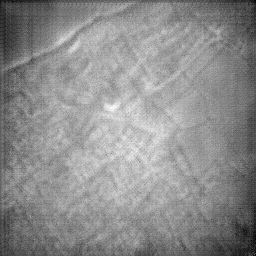
\includegraphics[width=\textwidth]{../figs/outputs/cycleGan/3.png}
  \end{subfigure}
  \hfill
  \begin{subfigure}[b]{0.19\textwidth}
      \centering
      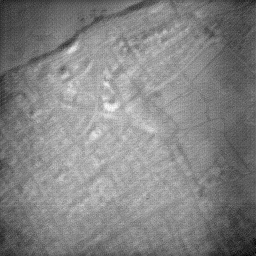
\includegraphics[width=\textwidth]{../figs/outputs/cut/3.png}
  \end{subfigure}
  \hfill
  \begin{subfigure}[b]{0.19\textwidth}
      \centering
      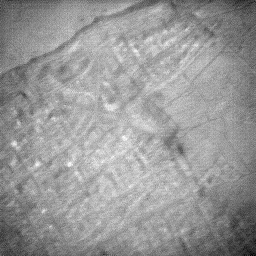
\includegraphics[width=\textwidth]{../figs/outputs/petit/3.png}
  \end{subfigure}
  \hfill
  \begin{subfigure}[b]{0.19\textwidth}
      \centering
      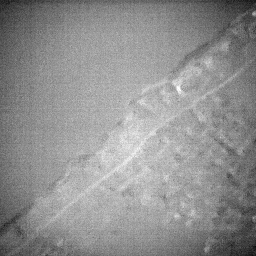
\includegraphics[width=\textwidth]{../figs/outputs/mono/1231.png}
  \end{subfigure}   
  
  % 3rd Row
  \centering
  \begin{subfigure}[b]{0.19\textwidth}
      \centering
      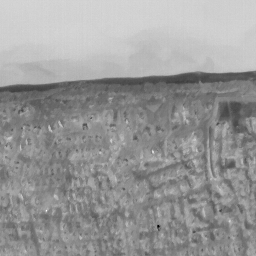
\includegraphics[width=\textwidth]{../figs/outputs/pan/13.png}
  \end{subfigure}
  \hfill
  \begin{subfigure}[b]{0.19\textwidth}
      \centering
      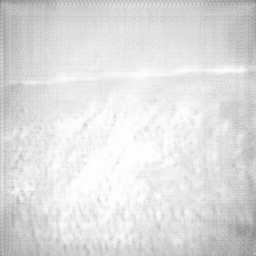
\includegraphics[width=\textwidth]{../figs/outputs/cycleGan/13.png}
  \end{subfigure}
  \hfill
  \begin{subfigure}[b]{0.19\textwidth}
      \centering
      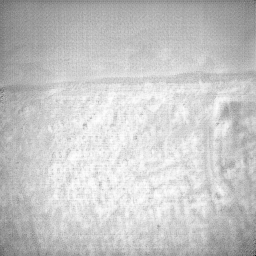
\includegraphics[width=\textwidth]{../figs/outputs/cut/13.png}
  \end{subfigure}
  \hfill
  \begin{subfigure}[b]{0.19\textwidth}
      \centering
      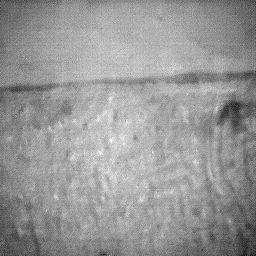
\includegraphics[width=\textwidth]{../figs/outputs/petit/13.png}
  \end{subfigure}
  \hfill
  \begin{subfigure}[b]{0.19\textwidth}
      \centering
      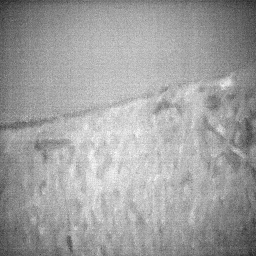
\includegraphics[width=\textwidth]{../figs/outputs/mono/399.png}
  \end{subfigure}    
  
  % 4th Row
  \centering
  \begin{subfigure}[b]{0.19\textwidth}
      \centering
      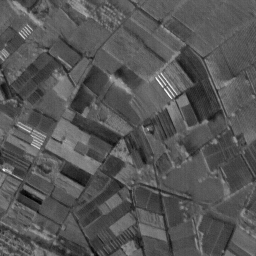
\includegraphics[width=\textwidth]{../figs/outputs/pan/50.png}
  \end{subfigure}
  \hfill
  \begin{subfigure}[b]{0.19\textwidth}
      \centering
      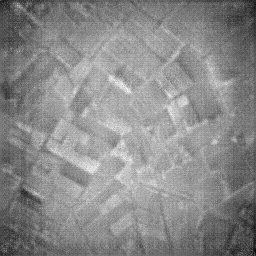
\includegraphics[width=\textwidth]{../figs/outputs/cycleGan/50.png}
  \end{subfigure}
  \hfill
  \begin{subfigure}[b]{0.19\textwidth}
      \centering
      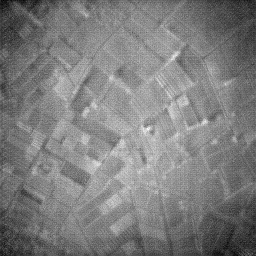
\includegraphics[width=\textwidth]{../figs/outputs/cut/50.png}
  \end{subfigure}
  \hfill
  \begin{subfigure}[b]{0.19\textwidth}
      \centering
      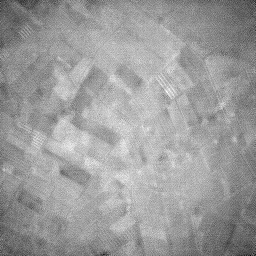
\includegraphics[width=\textwidth]{../figs/outputs/petit/50.png}
  \end{subfigure}
  \hfill
  \begin{subfigure}[b]{0.19\textwidth}
      \centering
      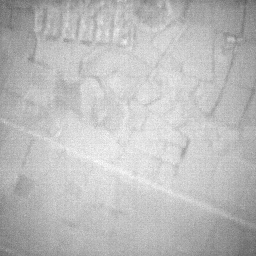
\includegraphics[width=\textwidth]{../figs/outputs/mono/397.png}
  \end{subfigure}    
  
  % 5th Row
  \centering
  \begin{subfigure}[b]{0.19\textwidth}
      \centering
      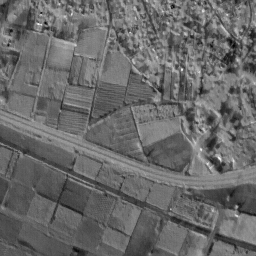
\includegraphics[width=\textwidth]{../figs/outputs/pan/112.png}
  \end{subfigure}
  \hfill
  \begin{subfigure}[b]{0.19\textwidth}
      \centering
      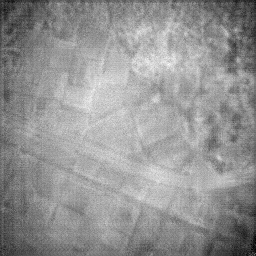
\includegraphics[width=\textwidth]{../figs/outputs/cycleGan/112.png}
  \end{subfigure}
  \hfill
  \begin{subfigure}[b]{0.19\textwidth}
      \centering
      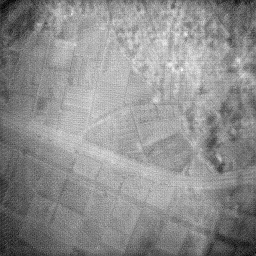
\includegraphics[width=\textwidth]{../figs/outputs/cut/112.png}
  \end{subfigure}
  \hfill
  \begin{subfigure}[b]{0.19\textwidth}
      \centering
      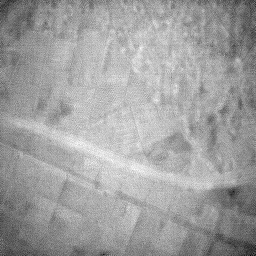
\includegraphics[width=\textwidth]{../figs/outputs/petit/112.png}
  \end{subfigure}
  \hfill
  \begin{subfigure}[b]{0.19\textwidth}
      \centering
      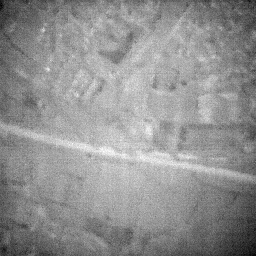
\includegraphics[width=\textwidth]{../figs/outputs/mono/563.png}
  \end{subfigure}    
  
  % last Row
  \begin{subfigure}[b]{0.19\textwidth}
      \centering
      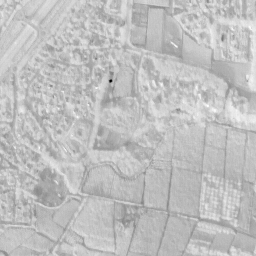
\includegraphics[width=\textwidth]{../figs/outputs/pan/7.png}
      \subcaption*{Pan (input)}
      \label{fig:pan}
  \end{subfigure}
  \hfill
  \begin{subfigure}[b]{0.19\textwidth}
      \centering
      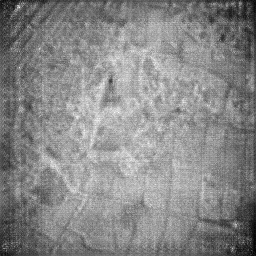
\includegraphics[width=\textwidth]{../figs/outputs/cycleGan/7.png}
      \subcaption*{CycleGAN (baseline)}
      \label{fig:cycleGan}
  \end{subfigure}
  \hfill
  \begin{subfigure}[b]{0.19\textwidth}
      \centering
      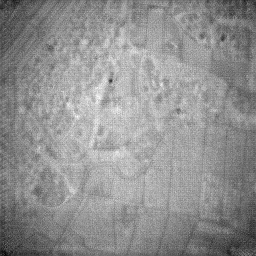
\includegraphics[width=\textwidth]{../figs/outputs/cut/7.png}
      \subcaption*{CUT (baseline)}
      \label{fig:cut}
  \end{subfigure}
  \hfill
  \begin{subfigure}[b]{0.19\textwidth}
      \centering
      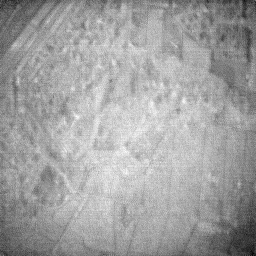
\includegraphics[width=\textwidth]{../figs/outputs/petit/7.png}
      \subcaption*{PETIT (ours)}
      \label{fig:petit}
  \end{subfigure}
  \hfill
  \begin{subfigure}[b]{0.19\textwidth}
      \centering
      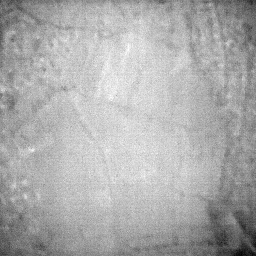
\includegraphics[width=\textwidth]{../figs/outputs/mono/1398.png}
      \subcaption*{Mono (ref)}
      \label{fig:mono}
  \end{subfigure}
  \caption{Qualitative comparison. (a) Panchromatic (Pan) input. (b) CycleGAN output. (c) CUT output. (d) PETIT output. (e) Real unpaired monochromatic image (Mono) for reference.}
  \label{fig:qual_res_sup}
\end{figure*}
% {\small
% \bibliographystyle{../ieee_fullname}
% \bibliography{../bib}
% }
\end{document}